\chapter{Requirements traceability}
This chapter traces the requirements to the user needs.

\section{Traceability matrix}
The traceability matrix ensures that all requirements fulfill a need. If a requirement does not fulfill a need, then it is redundant, or a new need has to be created.

\begin{figure}[H]
\centering

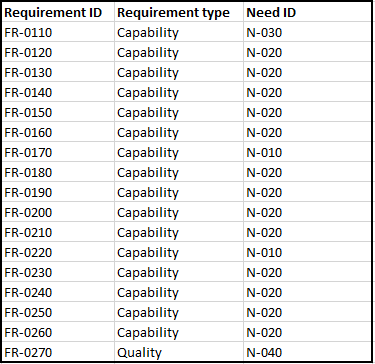
\includegraphics[scale=1]{Billeder/RTM.png}

\caption{Requirement tracebility matrix}
\label{RTM}
\end{figure}